\section{Auswertung}

Die Werte für die Induktivität \textbf{I}, den Festwiderstand \textbf{R} und den Kondensator \textbf{C}
für das Gerät (Gerät 1) was in diesen Versuch verwendet wurde sind:


\begin{align*}
    \textbf{I} = (16,87 \pm 0,05)\,\unit{\milli\henry} \,\,\,\,
    \textbf{R} = (67,2 \pm 0,1)\,\unit{\ohm} \,\,\,\,
    \textbf{C} = (2,060 \pm 0,003)\,\unit{\nano\farad}.
\end{align*}

\begin{flushleft}
    Wichtig hierbei zusagen ist noch, dass die Festwiderstände, kleine Wertunterschiede vorweisen die aber nicht sehr groß sind und deshalb beide Widerstände den Wert \textbf{R} haben. \\
    Die gewählte Frequenz $\textbf{\text{f}} = 250\,\unit{\hertz} $ mit einem verstellbaren Widerstand bis zu $10\,\unit{\kilo\ohm}$.
    Der Widerstand ist festgelegt auf $\textbf{\text{R}} = 0,2\,\unit{\kilo\ohm} $.
\end{flushleft}

\begin{center}
    X-Achseneinstellung (Zeit): $10\,\unit{\micro\second} $ pro Einheit \\
    Y-Achseneinstellung (Spannung):  $ 0,2\,\unit{\volt} $ pro Einheit \\
\end{center}

\newpage

\begin{table}
    \centering
    \caption{Die Tabelle der Amplitude in Zeitabhängigkeit.}
    \label{Tabelle1}
    \begin{tabular} {c  c}
        \toprule
        {$U_\text{c}  \mathbin{/}  \unit{\volt}$} &
        {$t \mathbin{/}  \mu \unit{\second}$} \\
        \midrule
        0,80  \pm 0,1  & 0 \\
        -0,60 \pm 0,1  & 10,0 \pm 0,1  \\
        0,58  \pm 0,1  & 20,0 \pm 0,1  \\
        -0,44 \pm 0,1  & 29,5 \pm 0,5  \\ 
        0,43  \pm 0,01 & 38,5 \pm 0,5  \\
        -0,32 \pm 0,02 & 48,5 \pm 0,5  \\
        0,32  \pm 0,01 & 58,5 \pm 0,5  \\
        -0,22 \pm 0,01 & 67,9 \pm 0,01 \\
        0,24  \pm 0,01 & 77,0 \pm 0,05 \\
        -0,18 \pm 0,01 & 86,0 \pm 0,5  \\
        0,17  \pm 0,05 & 97,0 \pm 0,01 \\
        \bottomrule
    \end{tabular} 
\end{table}

\begin{figure}
    \centering
    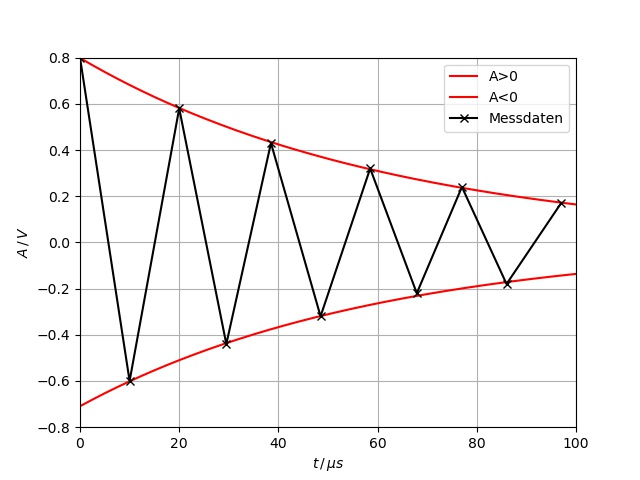
\includegraphics[width=90mm]{bilder/Ab10.jpeg}
    \caption{ Die Darstellung der Amplitude in Zeitabhängigkeit der Tabelle \ref{Tabelle1}. \label{Abbildung10} }
\end{figure}


\begin{align}
    \intertext{Die Einhüllende wird dargestellt in der Abbildung \ref{Abbildung10} mit den Werten aus der Tabelle \ref{Tabelle1} durch:}
    \text{A} = \text{A}_{0} \cdot e^{-2\,\pi\,\mu\,\text{t}}\,. \label{15}
    \intertext{Die Werte $\text{A}_{0}$ sowie $\mu$ lassen sich mit Hilfe einer Ausgleichsrechnung bestimmen:}
    \text{A}_{0} = (0,79 \pm 0,023)\,\unit{\ohm} \notag  \\
    \mu_{1}  = (0,0165 \pm 0,000940)\, \frac{1}{\unit{\second}} \notag
    \intertext{Der effektive Widerstand lässt sich durch umformen der oben genannte Funktion ausrechnen:}
    \text{R}_{\text{eff},1} = \mu_{1} \cdot 4\,\pi\,\cdot L = (0,00349 \pm 0,0016)\,\unit{\ohm}\,, \notag
    \intertext{ebenso die Abklingdauer}
    \text{T}_{\text{ex},1} = \frac{1}{2\,\pi\,\mu_{1}} = \frac{2\,\text{L}}{2\,\text{R}} = (9,645 \pm 0,321)\,\unit{\second} \notag
    \intertext{Vergleicht man nun die Werte des effektiven Widerstandes $\text{R}_{\text{eff},1}$ und den vorgegebenen Widerstand $\text{R} = (67,2 \pm 0,1)\,\unit{\ohm}$, so fällt auf, dass es eine Differenz von $-67,196\,\unit{\ohm}$ vorhanden ist.} \notag
\end{align}

\begin{align*}
    \intertext{Um den aperiodischen Widerstand im Grenzfall zu untersuchen, wurde der Graph so eingestellt, wie in Abbildung {\ref{Abbildung8}} zu sehen.
    Durch das Ablesen ergibt sich für $\text{R}_{\text{ap}}$ einen Wert von}
    \text{R}_{\text{ap}} = 2,2\,\unit{\kilo\ohm} = 2,2 \cdot 10^3\,\unit{\ohm}\,.
    \intertext{Der theoretische Wert lässt sich wie in der Formel (\ref{5}) bestimmen:}
    \text{R}_{\text{ap}} = \sqrt{\frac{4\,\text{L}}{\text{C}}} = (5723 \pm 0,013) \cdot 10^3\,\unit{\ohm}.
    \intertext{Die Abweichung beträgt 3,523 \unit{\kilo\ohm}, welches sich auf weitere Bauelemente zurückführen lassen kann, da wir nur $\text{R}_{1}$ bzw. $\text{R}_{2}$ gegeben haben, wurden andere Widerstände vernachlässigt.
    Somit haben wir es mit einem systematischen Fehler zu tun.
    Da $\text{R}_{\text{ap}}$ empirisch bestimmt wurde, können (größere) Messfehler auftreten.} 
\end{align*}


\begin{table}[H]
    \centering
    \caption{Frequenzabhängigkeit der Kondensatorspannung.}
    \label{Tabelle2}
    \begin{tabular} {c   c   c   c}
        \toprule
        {$ \text{U}_{0} \mathrm{/} \unit{\volt} $} &
        {$ \text{U}_{\text{C}} \mathrm{/} \unit{\volt} $} &
        {$ \frac{\text{U}_{\text{C}}}{\text{U}_{0}} $} &
        {$ \text{f} \mathrm{/} \unit{\kilo\hertz} $}\\
        \midrule
        4,8 & 0,52 & 0,1083 & 5  \\
        4,8 & 0,56 & 0,116  & 10 \\
        4,8 & 0,68 & 0,141  & 15 \\ 
        4,2 & 1,15 & 0,273  & 20 \\
        4,2 & 1,29 & 0,307  & 22 \\
        4,2 & 1,60 & 0,380  & 24 \\
        4,2 & 1,89 & 0,45   & 26 \\
        4,2 & 1,70 & 0,404  & 28 \\
        4,2 & 1,30 & 0,309  & 30 \\
        4,2 & 1,00 & 0,238  & 32 \\
        4,2 & 0,80 & 0,190  & 34 \\
        4,2 & 0,61 & 0,145  & 36 \\
        4,2 & 0,505& 0,120  & 38 \\
        4,2 & 0,50 & 0,119  & 40 \\
        \bottomrule
    \end{tabular} 
\end{table}


\begin{figure}[H]
    \centering
    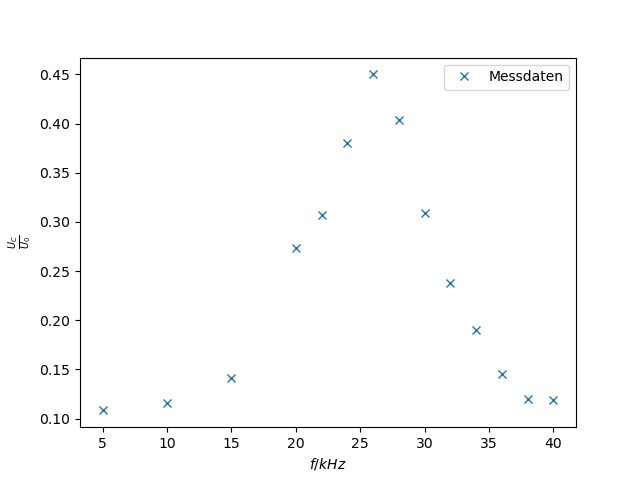
\includegraphics[width=90mm]{bilder/Ab11.jpeg}
    \caption{Darstellung der Werte $\frac{\text{U}_{\text{C}}}{\text{U}_{0}}$ in Frequenzabhängigkeit aus der Tabelle \ref{Tabelle2}. \label{Abbildung11} }
\end{figure}

\begin{align}
    \intertext{Die Güte q wurde experimentell bestimmt zu: $ \text{q}_{\text{e}} = 0,45 $.}
    \intertext{Man betrachte, dass unsere Spannung $ \text{U} = 2\,\unit{\volt}\mathbin{/}\text{Div} $, sowie $ \text{U}_{\text{C}} = 0.5\,\unit{\volt} \mathbin{/}\text{Div} $ bzw. $ 0.2\,\unit{\volt} \mathbin{/}\text{Div}  $
    am Oszilloskop eingestellt wurde. Der theoretische Wert lässt sich durch die Gleichung}
    \text{q} = \frac{1}{\omega_{0}\,\text{RC}} \quad mit \quad \omega_{0} = \sqrt{\frac{1}{\text{LC}}} \label{16}
    \intertext{ermitteln zu}
    \text{q} = 42,58 \pm 0,15 \quad mit \quad \text{R}_{2} = 67,2 \notag  \\
    Abweichung: \frac{\text{q}_{\text{exp}} - \text{q}_{\text{theo}}}{\text{q}_{\text{theo}}}\,. \notag \\
    \text{Die Abweichung hierbei beträgt}\,\, -98\%\,. \notag
    \intertext{Anschließend wird unsere Resonanzkurve mit einer linearen Gerade ergänzt. Die Gerade befindet sich bei}
    \frac{\text{U}_{\text{C}}}{\text{U}_{0}} = \frac{\text{q}_{\text{e}}}{\sqrt{2}} = 0,318\,. \notag
\end{align}

\begin{align*}
    \intertext{Zudem werden Halbwertsbreiten an den Punkten, welche sich mit dem Graphen kreuzen, aufgestellt.
    Der ermittelte Wert lautet}
    \nu_{+} - \nu_{-} = 7 \cdot 10^3\,\unit{\hertz} \\
    \intertext{Theoretisch: mit der Formel (\ref{14}):} 
    \nu_{+} - \nu_{-} = \frac{117\,\unit{\ohm}}{16,87\,\unit{\milli\henry}} = (6,9 \pm 0,000012) \cdot 10^{3}\,\unit{\hertz}  \notag\\
    \text{Die Abweichung hierbei beträgt}\,\, 1,15\%\,.
\end{align*}

\begin{align}
    \intertext{Die Phasenverschiebung der ersten drei gemessenen Werte beläuft sich bei einer Frequenz von $15\,\unit{\hertz}$ auf $10\,\unit{\micro\second}$. 
    Die Phasenverschiebung der restlichen gemessenen Werte beläuft sich bei einer Frequenz von $30\,\unit{\hertz}$ auf $6\,\unit{\micro\second}$.
    Eine ganze Phase beträgt $20\,\unit{\micro\second}$}
    \intertext{Die Berechnung einer Phase geht über die Formel}
    \left(\frac{\text{A}}{\text{B}} \right) \cdot 360°\,. \label{17}
    \intertext{Wobei \textbf{A} $D/V$ zwischen den Kästchen ist und \textbf{B} die komplette Phase ist.} \notag
\end{align}


\begin{figure}[H]
    \centering
    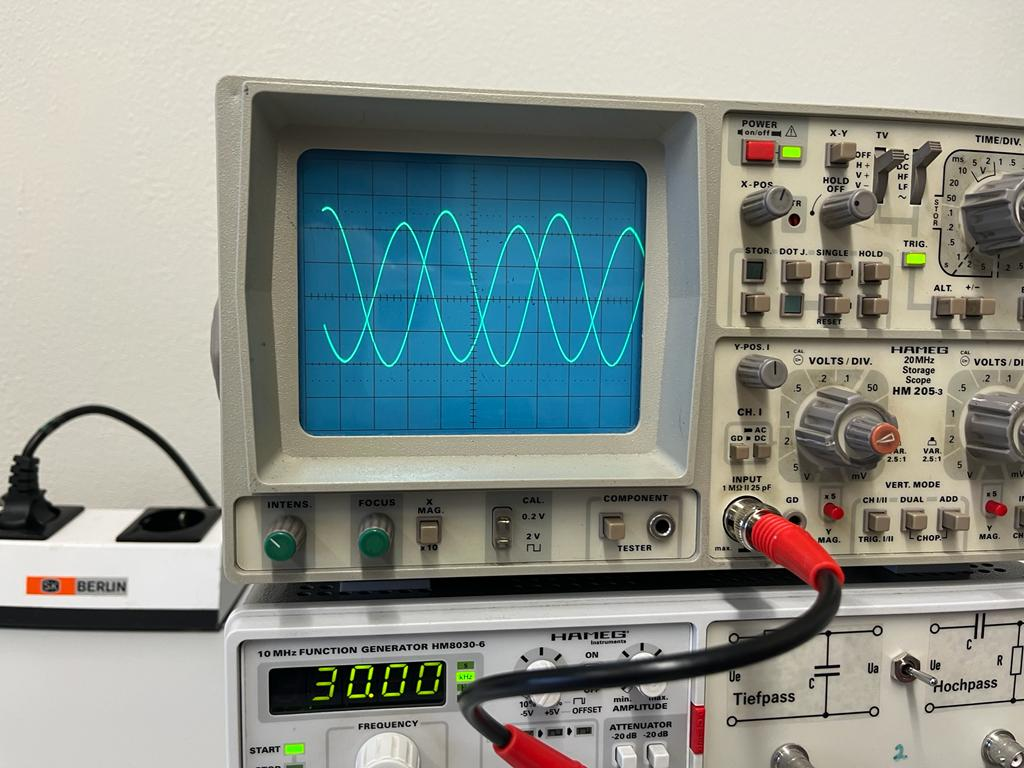
\includegraphics[width=76mm]{bilder/Ab12.jpeg}
    \caption{Die Phasenverschiebung am Oszilloskop verbildlicht.\label{Abbildung12}}
\end{figure}

\begin{table}[H]
    \centering
    \caption{Frequenzabhängigkeit der Kondensatorspannung.}
    \label{Tabelle3}
    \begin{tabular} {c  c  c}
        \toprule
        {$ \nu \mathbin{/} 10^{3}\,\unit{\hertz} $} &
        {$ \text{t} \mathbin{/} \mu \unit{\second}$}  &
        {$ \phi \mathbin{/} \unit{\degree} $}\\
        \midrule
        15 & 1 & 17,9  \\
        30 & 6 & 107   \\
    \end{tabular} 
\end{table}



